\section{SDC methods}
\label{Theory:SDCMethods}

We will describe now some of the most common methods and mechanisms used in SDC applications to anonymize data or provide privacy preserving data releases.

\subsection*{Notation}

We assume the following notation for the subsequent method descriptions:

\begin{itemize}
	\item
	The original dataset is the matrix $X$, with $n$ rows (samples) and $m$ attributes or variables. Therefore, the $x_{ij}$ element of the dataset denotes the value that the $j$-th attribute takes in the $i$-th row for any $1 \leq i \leq n$ and $1 \leq j \leq m$.
	
	\item
	The anonymized (protected) dataset is named $X'$.
\end{itemize}

\subsection{Noise Addition}
\label{Theory:SDCMethods:NoiseAddition}

Noise addition or \textit{additive noise masking} is a fairly simple method that is based on the addition of gaussian noise to data, thus randomly distorting its values and difficulting re-identification of individuals. The main additive noise algorithms in the literature are~\citep[p. 54]{Hundepool:StatisticalDisclosureControl}:

\begin{itemize}
	\item
	Uncorrelated noise addition.
	\item
	Correlated noise addition.
	\item
	Noise addition and linear transformation.
	\item
	Noise addition and non-linear transformation.
\end{itemize}

We will only cover the first couple of methods, because of the inherent difficulty of the latter, both in its theoretical basis and its practical implementation, which renders them not suitable for the needs of this project.

\subsubsection{Uncorrelated noise addition}

Masking by additive noise the $j$-th variable of an original dataset $X$ yields an anonymized dataset $X'$ such that

\begin{equation}
x_{ij}' = x_{ij} + \epsilon\ \ \ \text{for}\ 1 \leq i \leq n
\end{equation}

where $\epsilon$ is drawn from a random variable $\varepsilon_j \sim N(0,\sigma_{\varepsilon_j}^2)$. The general assumption is that the variances of each $\varepsilon_j$ are proportional to those of the original variables, this is, if $\textrm{Var}(X_j) = \sigma_j^2$ is the variance of the $j$-th attibute of the dataset $X$, then $\sigma_{\varepsilon_j}^2 := \alpha\sigma_j^2$.

While this method preserves means and covariances, it is, unfortunately, not able to preserve variances nor correlation coefficients.

\subsubsection{Correlated noise addition}

This method is aimed to also preserve correlation coefficients, with respect to \textit{uncorrelated} noise addition. The main difference with the previous mechanism is that the covariance matrix of the errors is now proportional to the covariance matrix of the data: $\varepsilon \sim N(0,\Sigma_\varepsilon)$, where $\Sigma_\varepsilon = \alpha\Sigma$.

Masking by correlated noise addition provides data with higher analytical utility than masking using uncorrelated noise, as long as $\alpha$ is revealed to the data user. However, the low level of protection yielded by this method and the previous one render them as not very useful for truly important SDC applications.

\subsection{Microaggregation}
\label{Theory:SDCMethods:Microaggregation}

Originally described for continuous (numerical) data, microaggregation is a family of SDC methods that, in the most general form, consist of making homogeneous groups of $k$ or more individuals (rows) from within the $X$ dataset to later replace their values with aggregated ones, this is, averages, computed on the groups themselves. These grouped and aggregated records conform the resulting $X'$ release dataset.

Two main approaches are taken when considering microaggregation techniques: \textit{univariate} and \textit{multivariate} microaggregation. The difference remains in the number of variables used to perform the \textit{clustering} phase of the method: a single variable and multiple attributes, correspondingly. As can be assessed in the literature, the univariate approach causes either a very high information loss or a very high disclosure risk, thus not being appropriate for normal SDC uses~\citep[p. 63]{Hundepool:StatisticalDisclosureControl}. On the other hand, multivariate microaggregation, proposed by~\citet{Domingo:PracticalMicroaggregation}, is considered an excellent protection method and, as such, we will focus on this approach.

It is important to note that this family of techniques are directly related to $k$-anonymity, as proved in~\citet{Domingo:KAnonMicroagg}.

\subsubsection{Partition}

The first and most computational complex task to do in a microaggregation method is to partition the dataset into $g$ groups of size at least $k > 1$, which is, indeed, a \textit{clustering} task. This proves to be quite difficult, but an optimal solution approximation with respect to information loss was already given in~\citep{Domingo:KAnonMicroagg} and further refined in~\citet{Domingo:MuAproxPolyTimeMicroagg}.

The aim of these partition methods is to find the optimal $k$-partition that maximizes within-group homogeneity. Following~\citet{Domingo:PracticalMicroaggregation}, a practical information loss measure for microaggregation, relatively common in the clustering literature, is the ratio of within-group homogeneity over the total sum of squares (the sum of \textit{within} and \textit{between} group homogeneity)

\begin{equation}\label{eq:clustering-info-loss}
L = \frac{SSE}{SST}
\end{equation}

The within-group homogeneity ($SSE$) is defined as

\begin{equation}
SSE = \sum_{i=1}^{g} \sum_{j=1}^{n_i} (x_{ij} - \mathbf{\bar{x}_i})^2
\end{equation}

where $g$ denotes the total number of groups of $n_i$ elements each and $\mathbf{\bar{x}_i}$ denotes the $i$-th group centroid. The between-groups sum of squares, $SSA$, is

\begin{equation}
SSA = \sum_{i=1}^{g} n_i (\mathbf{\bar{x}_i} - \mathbf{\bar{x}})^2
\end{equation}

where $\mathbf{\bar{x}}$ is the average vector over the whole dataset. The total sum of squares is, then, $SST = SSE + SSA$.

Because microaggregation replaces values in a group by the group centroid, if we recall~\eref{eq:clustering-info-loss}, it follows that the higher the within-group homogeneity, the lower the information loss is. Both the MDAV~\citep{Domingo:KAnonMicroagg} (Maximum Distance to Average Vector) and $\mu$-Approx~\citep{Domingo:MuAproxPolyTimeMicroagg} algorithms are built to partition the dataset into groups, while minimizing information loss, exploiting the previous theoretical result.

\subsubsection{Aggregation}

The aggregation step is the simplest of the ones that take place in a microaggregation setting: for each group $g$ of at least $k$ records and for each attribute $1 \leq j \leq m$, an \textit{aggregate} $\gamma$ is computed among the values of the $j$-th variable for the records in the group. This aggregate is then imputed to each record for its $j$-th attribute.

Concerning the types of variables that are aggregated~\citep{Domingo:KAnonMicroagg}:

\begin{itemize}
	\item
	\textbf{Continuous attributes:} the aggregated value correponds with the arithmetical mean of the selected values.
	\item
	\textbf{Categorical attributes:} the aggregated value should either be the median or the mode of the selected values.
\end{itemize}

\subsection{Rank Swapping}
\label{Theory:SDCMethods:RankSwapping}

Also a fairly simple SDC method, the basic idea behind data swapping and its refinement, \textit{rank swapping}, is to transform a dataset by exchanging values of confidential variables in such a way that marginals are maintained. The method works as follows:

First, values of a variable $j$ are ranked in ascending order, this is, they are \textit{sorted}. Each ranked value is then swapped with another ranked value, randomly chosen within a restricted range. This range is controlled by an input parameter $p$, normally denoting that swapped values cannot differ more than $p\%$ of the total number of records. This procedure is applied for every variable in the dataset.

\subsection{Laplace Mechanism}
\label{Theory:SDCMethods:LaplaceMechanism}

We recall now the context of differential privacy to discuss a relatively extended method that is designed to achieve this privacy preserving guarantee. However, this technique is restricted to a particular family of data release functions. More precisely, it can only be applied to functions that provide a \textit{numerical} answer, like counting queries, for example. To understand this method, called \textit{Laplace mechanism}, we must review first the concept of \textit{global sensitivity} of a function.

\begin{definition}~(Neighbour datasets)
Given two datasets from a universe of datasets, $D_1, D_2 \in \mathcal{D}$, we call them \textit{neighbours} if they differ in just one record, which we indicate using the notation $|D_1 \Delta D_2| = 1$.
\end{definition}

\begin{definition}~(Global Sensitivity of a function)
We define the global sensitivity of a numerical function $f : \mathcal{D} \rightarrow \mathbb{R}^w$, with $w \in \mathbb{N}^+$, over the universe of datasets $\mathcal{D}$, as
\begin{equation}
\Delta(f) = \max_{\substack{D_1, D_2 \in \mathcal{D} \\ |D_1 \Delta D_2| = 1}} \lVert f(D_1) - f(D_2) \rVert_{1}
\end{equation}
\end{definition}

As we will now see, the Laplace mechanism is just a noise addition masking method, where the sensitivity of the release function $f$ drives the amount of noise being added to the response of $f$: the higher the sensitivity of the function, the higher the amount of noise added. If $f$ is applied to a dataset $D_1$ and then to a neighboring dataset $D_2$, if $f$ changes a lot, it means that we will have to add more noise to probably obtain the same output.

\begin{definition}~(Laplace mechanism)
Given a database $D \in \mathcal{D}$ and a function $f : \mathcal{D} \rightarrow \mathbb{R}^w$, with $w \in \mathbb{N}^+$ and global sensitivity $\Delta$, an $\varepsilon$-differential privacy mechanism $\mathcal{M}$ for releasing $f$ is to publish
\begin{equation}
\mathcal{M}(D) = f(D) + L
\end{equation}
where $L$ is a vector of random variables each drawn from a Laplace distribution $Lap(0, \frac{\Delta(f)}{\varepsilon})$.
\end{definition}

This mechanism ensures that $\varepsilon$-differential privacy is achieved for the release function $f$, as can be assessed in~\citet{Leoni:NonInteractiveDiffPriv} and~\citet{Domingo:EnhancingDiffPrivMicroaggregation}.

\subsubsection*{Laplace distribution}

On a quick note to understand the kind of noise being added through the Laplace mechanism, a Laplace distribution $Lap(\mu, b)$ has \textit{location} $\mu$ (which could be understood as the mean or the location of the \textit{peak} of the PDF of the distribution) and \textit{scale} parameter $b$. This last parameter is the one used to adjust the amount of perturbation the data or release method will receive.

\begin{figure}[h]
	\centering
	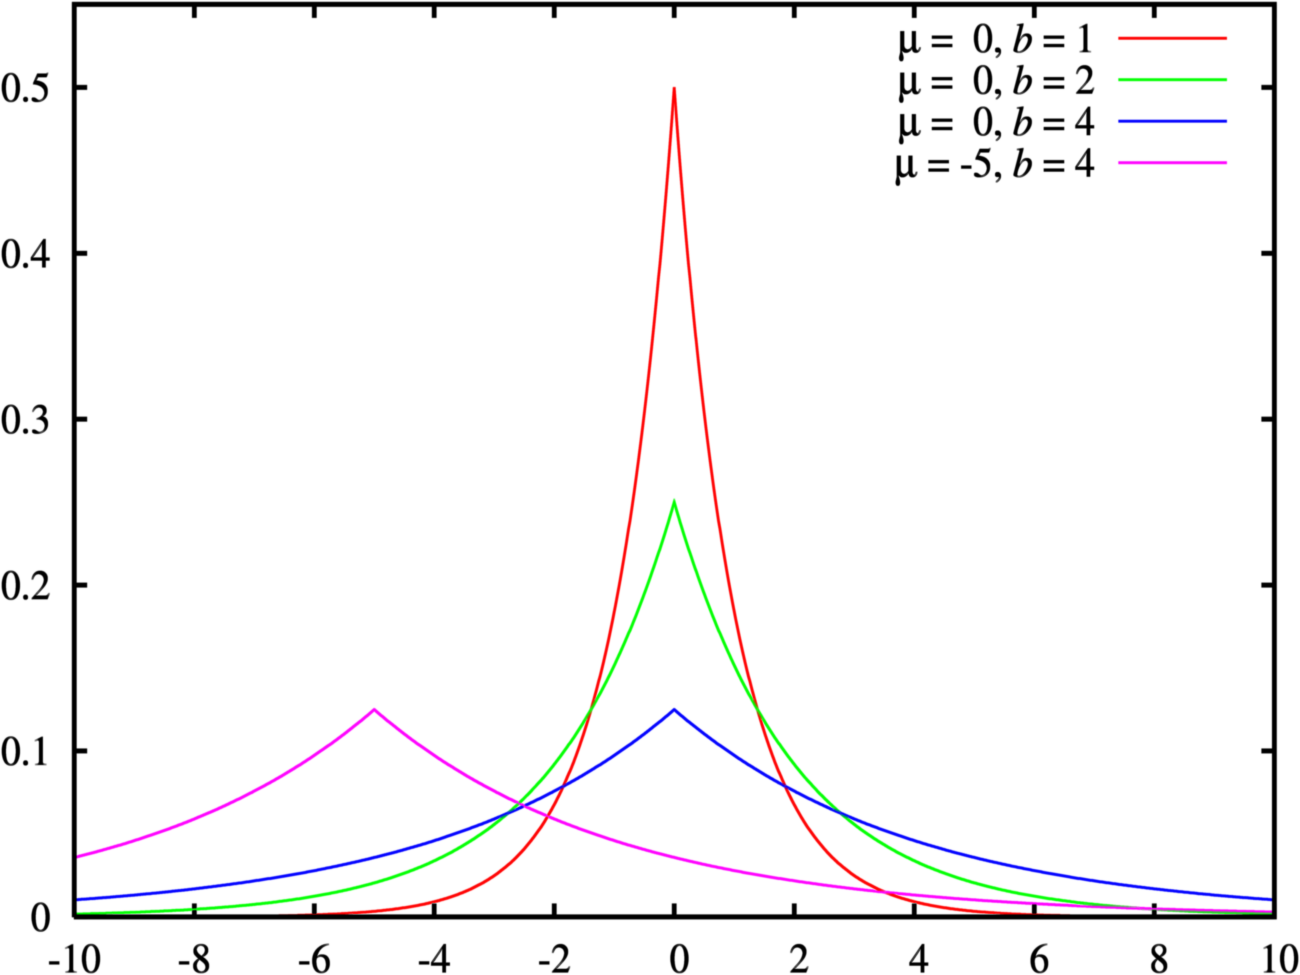
\includegraphics[width=0.5\linewidth]{figures/laplace-pdf.png}
	\label{fig:laplace-pdf}
	\caption[Laplace distribution.]{Laplace distribution probability density function (PDF). Source: Wikipedia~\cite{web:Wiki:LaplaceDist}}
\end{figure}

The density function of the Laplace noise, also called \textit{double exponential}, is

\begin{equation}
P(x|\mu,b) = \frac{1}{2b}\exp(-\frac{|x-\mu|}{b})
\end{equation}






